\lhead{\emph{System Design}}
\chapter{System Design}

\section{System Components}
In this chapter we will provide an overview \autoref{fig:systemComponents} of the components of the system and their function. The overall system is divided into three components remote data collection, data transport and, the server processing and storage.  It is presumed that the remotes have varying locations (although they may stay in a single place for months or years). Remotes are not specifically tied to any geography.  They may be it marine or land based. In this discussion, examples are assumed to be a marine application.  

\begin{figure}
\centering
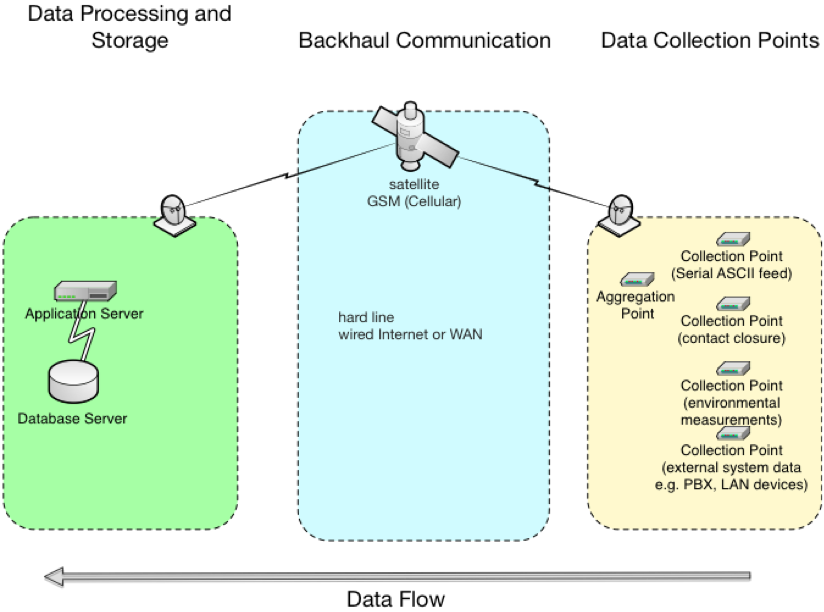
\includegraphics{Figures/systemComponentOverview}
\caption{System Components}
\label{fig:systemComponents}
\end{figure}
\section{Data Collection Component}

The layout of the data collection component tiered and resides fully on the remote site.  The devices that act as collection points are known in our system as nodes.  They are installed on-board with the tasks to receive, secure and transmit the data.  A remote site must house at least one node but may have multiple nodes installed.  Each node, in turn, is comprised of one or more data inputs called tendrils.  A tendril is a single source of data which reports directly to the node. 

\subsection{Nodes}

The node uses a small on-board device which is capable of running a general use operating system. For our mock up node, a BeagleBoard\cite{Anonymous:zgMDnVpL} brand embedded device is used.  The node is designed to have a small resource footprint with CPU, memory and storage capacity restricted and cost effective.  The device is configured with 512M of RAM, a single code CPU, and 1 Gig of SSD disk storage.  The CPU draws very little power and produces minimal heat.  This relieves a requirement for a fan in most applications and results in a device with no moving parts.  

A node may receive inputs from a variety of sources.  Each node's id is unique throughout the system.  With a unique id it is possible to have many nodes installed on a single remote site and across sites and nodes can be migrated to other sites. This proves useful in the case that a datasource is moved. For instance if a cargo container is transported to another ship. 
In our reference implementation we will limit to a single node with multiple simulated inputs.  These inputs are referred to as tendrils that are tasked to provide the events to the node.  The node will accept to a variety of different tendrils and collect their event information.  

\begin{figure}
    \centering
    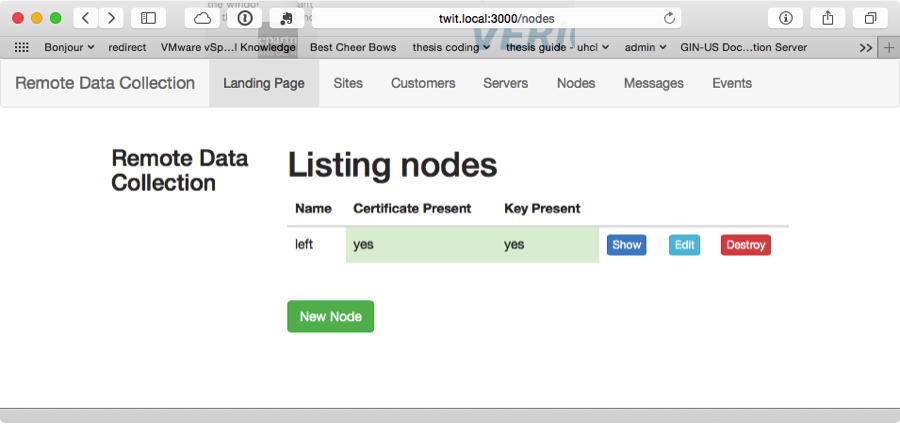
\includegraphics[scale=.9, angle=0]{Figures/interfaceNodes}
    \caption[Nodes Interface]{Web Based Interface for Node Management}
    \label{fig:interfaceNodes}
\end{figure}

\subsection{Tendrils}
The idea of the tendril is one of flexibility. 
It is designed with an abstraction layer based on the REST protocol. A wide variety of information is made possible by this design. 
Example types include Environmental, State Change Detection, Location, and events sent by intelligent systems.  
More specific examples include: ambient temperature, humidity, door openings and closures of a cargo container, GPS position, wave height, wind speed and sophisticated system activities such as phone calls and email activity. We create three types of tendril inputs although any number may be possible. Contact closure, serially attached streams, and intelligent system messages present an overview of what is possible. 
\subsubsection{Contact Closure}
Contact closures\cite{OmegaEngineeringInc:vi} in this context would have a circuit connected to a relay on a door, for example. Opening the door also creates an open circuit is detected by our agent. The event is recorded and secured on the agent with a timestamp and position if available. The purpose of such a measurement is to detect a container being accessed. The event, once processed, is compared against a policy of access that determines if the access was authorized. The converse of this is to detect events that are scheduled to occur. For example detection of a fuel cap being removed on a generator to indicate it was inspected. \autoref{fig:contactClosure} Contact closure relays are low cost devices that can be configured as a tendril\cite{Anonymous:wa}.
\begin{figure}
\centering
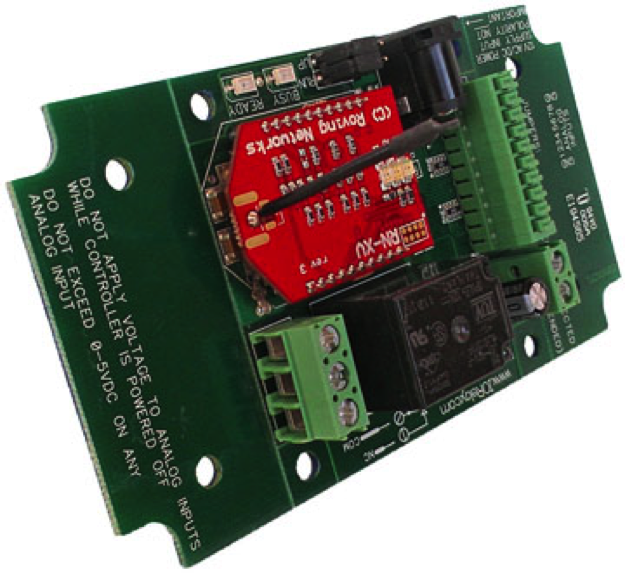
\includegraphics{Figures/contactClosure}
%\caption{Contact Closure - RelayPros R110PL_WIFI WiFi Relay}
\caption{Contact Closure - RelayPros Wifi Relay}
\label{fig:contactClosure}
\end{figure}
\subsubsection{Serially Attached Systems} 
Serially attached systems are considered to be systems attached via an RS–232 or similar pinned connection. They are devices that have a serial console connect which provides either a stream of character data or an updated status screen. An example is a GPS device which provides a NEMA string. A device in this configuration has a consistent stream of ASCII data using a standard protocol. GPS positioning coordinates as well alarms and electronic fence data are sent down the serial link to the attached node. Within the node, as with all devices, the stream data is secured in messages for transmission to the storage systems.
\subsubsection{Intelligent Systems}
We recognize a third category of tendril data sources termed intelligent systems. They have the ability to process, compile and digest their information before collection. They have significant processing power and can transmit over a local network to the local node.  
Examples of these are VoIP call managers, routing, switching, and WiFi infrastructure, and servers.  These can record call detail records for from call managers, routers and infrastructure log data, and diver / ROV  \cite{Christ:2011vn} video systems.
Potential use cases include but are certainly not limited to: Logging Environmental Systems Call Manager Systems, Email, and Cell phone usage
The end result of all this information collection with the remote is the standard interface that feeds the message. Upon. The remote upon receiving an input it will take me information contained and security and the message Block. These message locks are then either transferred immediately or stored and transferred once the system is online.
During the Deepwater Horizon explosion, many elements of data were generated leading up to the explosion itself. 
Much of this data was from the phone system and cellular network. Both of these could have been captured and transmitted up to the point that connectivity was lost. 


\section{Transmission}
The transmission component of the system, also referred to as the backhaul, can be provided by a number of network topologies and technologies. Therefore we can make few assumptions about it’s quality, bandwidth, or availability. The system therefore treats the transmission component as a generic pipe. The one assumption that we do make is that the connection must be available before the node resources are exhausted. This will vary depending on the application but generically we expect communication to be resumed available every 24 to 48 hours. Practical expectation is that connectivity would be more frequent and stable.

This backhaul link is also assumed to be inherently insecure. Public networks such as the Internet and cellular phone networks will be routinely used. Therefore all security is managed within the message block itself. Key exchange (key agreement) is provided using a pre-shared, symmetric key. In this model the message processing does not require the transmission link to be online when messages session key is created.

\section{Storage and Processing}
The storage and processing component of the system is the server that lives within the data center. The site would be a corporate installation owned and controlled by the end user. Security of the physical system and access to the operating system are assumed.  Messages received by the server are decrypted and placed into the database. Depending on the sensitivity of the message appropriate database level encryption can be used for increased protection and prevents access by an authorized user should the system be breached. 

The storage and processing component of the system is composed of three functional pieces. At its base provides a data store for the messages to be decrypted and stored. and available for processing. Secondly, it provides the business logic interface for configured rules and their thresholds. Finally it is the user interface for provisioning and management, and key management the node devices. 

\section{Reporting}
As part of the storage and processing we expect to produce a geographic mapping application \autoref{fig:interfaceMap} to show the position of the nodes as they traverse the. 
Popup values such as online / off-line, number of messages received, and time since last contact. The interface should also provide the ability for the user to correlate events. E.g. correlate by time, by a fleet, by system type. 

\begin{figure}
\centering
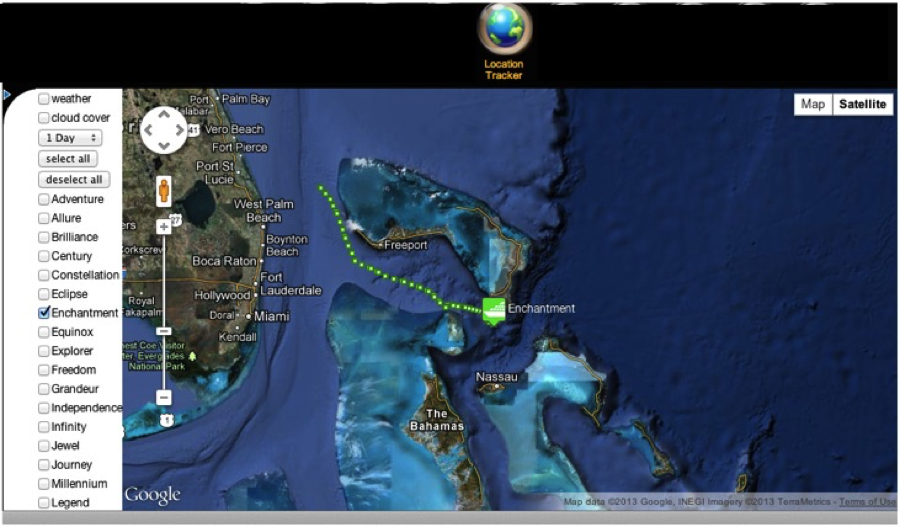
\includegraphics[scale=.9]{Figures/interfaceMap}
\caption{Map Interface}
\label{fig:interfaceMap}
\end{figure}